\documentclass[a4paper,12pt]{book}
\usepackage[utf8]{inputenc}
\title{}
\author{Rachel Morris}
\date{\today}

\usepackage{rachwidgets}
\usepackage{fancyhdr}
\usepackage{lastpage}
\usepackage{dirtree}
\usepackage{boxedminipage}

\setcounter{chapter}{7}
\setcounter{section}{0}
\newcommand{\laChapter}{7.1 Graph Theory\ }

\newcommand{\laClass}{CS 211\ }
\newcommand{\laSemester}{Fall 2017\ }
\newcounter{question}

\pagestyle{fancy}
\fancyhf{}
\lhead{CS 211 Exercise}
\chead{Fall 2017}
\rhead{Ch \laChapter}
\rfoot{\thepage\ of \pageref{LastPage}}
\lfoot{\scriptsize Compiled by Rachel Morris, last updated \today}

\renewcommand{\headrulewidth}{2pt}
\renewcommand{\footrulewidth}{1pt}

\begin{document}

    %\toggletrue{answerkey}
    \togglefalse{answerkey}


    \notonkey{
    %- Team Info ------------------------------------------------------%

    \paragraph{Team name:}

    ~\\~\\
    Please write down all people in your team. ~\\

    % table %
    \begin{tabular}{ p{6cm} p{6cm} }
        1. & 2. \\ \\
        3. & 4.
    \end{tabular}
    % table %
    ~\\

    \hrulefill
    \subsection*{Grading}

    \begin{center}

        \begin{tabular}{ | l | l | l | }
            \hline
            \textbf{ Question } & \textbf{ Score } & \textbf{ Max } 
            \\ \hline
            1 &  & 4     \\ \hline
            2 &  & 4     \\ \hline
            3 &  & 2     \\ \hline
            & &  \\ \hline
            Total & & 10
            \\ \hline
        \end{tabular}
    \end{center}
    }{}

    \section{Graph Theory}

    \subsection{Terminology}

        Since we're introducing a new concept, Graph Theory,
        we need to go over the various terms so that we
        can communicate about these graphs properly.

        \begin{intro}{\ }
            \begin{itemize}
                \item   \textbf{Graph:} A graph is a type of diagram that contains \textit{vertices} (aka nodes) and \textit{edges}.

                \begin{center}
                    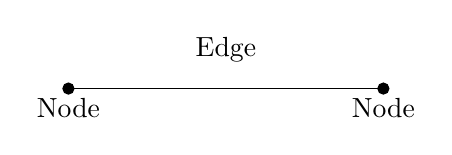
\begin{tikzpicture}
                        \filldraw (-2,0) circle (2pt) node[align=left, below] {Node};
                        \filldraw (2,0) circle (2pt) node[align=left, below] {Node};
                        \draw (-2,0)   to (2,0);
                        \node [fill=none] at (0,0.5) {Edge};
                    \end{tikzpicture}
                \end{center}

                \item   \textbf{Node:} A vertex of the graph, drawn as a dot.
                    \begin{itemize}
                        \item   \textbf{Adjacent nodes:} Two nodes that are connected by an edge.
                    \end{itemize}

                \item   \textbf{Edge:} A line that connects two nodes together.
                    \begin{itemize}
                        \item   \textbf{Parallel edges:} Two edges that have
                            the same two endpoints.
                        \item   \textbf{Loop:} An edge that begins and ends at
                            the same node, creating a loop.
                    \end{itemize}

                \begin{center}
                    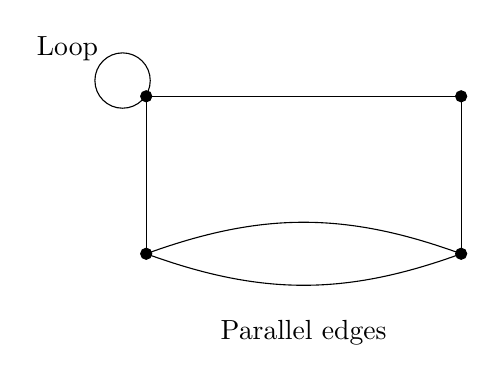
\begin{tikzpicture}
                        \filldraw (-2,0) circle (2pt);
                        \filldraw (2,0) circle (2pt);
                        \filldraw (-2,2) circle (2pt);
                        \filldraw (2,2) circle (2pt);
                        \draw (-2,0)   to[bend left=-20] (2, 0);
                        \draw (-2,0)   to[bend left=20] (2, 0);
                        \draw (2,0) -- (2,2) -- (-2,2) -- (-2, 0);
                        
                        \node [fill=none] at (0,-1.0) {Parallel edges};
                        \node [fill=none] at (-3,2.6) {Loop};
                        \draw (-2.3,2.2) circle (10pt);
                    \end{tikzpicture}
                \end{center}
            \end{itemize}

        \end{intro}

		\newpage
					
        \begin{intro}{\ }
            \begin{itemize}
                \item   \textbf{Walk:}	 A series of alternating
                		nodes and edges, traversing between adjacent nodes.
                    \begin{itemize}
                        \item   \textbf{Closed walk:} When the beginning
	                        and ending node of a walk are the same.
						\item  \textbf{Length of a walk:} The amount
							of edges in the walk.
						\item \textbf{Trivial walk:} A walk of length 0.
                    \end{itemize}
                    
                \item   \textbf{Trail:}	A walk with no repeated edges.
                \item   \textbf{Path:} A walk with no repeated vertices.
                \item   \textbf{Circuit:} A closed trail.
                \item   \textbf{Trivial circuit:} A circuit with one vertex and no edges.
                \item   \textbf{Eulerian:} A trail or circuit where every edge is traversed.
                \item   \textbf{Cycle:} A nontrivial circuit where the only repeated node is the first/last one.
            \end{itemize}

        \end{intro}


\end{document}
